\setcounter{chapter}{5}
\chapter{\acs{fastPLI} package}
\label{chap:Software}
% 
% 
\includegraphics[width=.075\textwidth]{gfx/Scihub_raven.png}
% \cleanchapterquote{Journal paywalls are an example of something that works in the reverse direction, making communication less open and efficient.}{Alexandra Elbakyan}{}
% % 
% % \tikz[remember picture,overlay] \node[inner sep=0pt] at (0,0){
\includegraphics[height=7em]{gfx/Scihub_raven.png}};
% % \hspace{-10em}
% % \clearpage opacity=0.3,
% 
% 
%  
\section{Package}
% 
The previous chapters descried algorithms for building dense \ac{WM} fiber models (see \cref{chap:sof:modelling}) and the simulation of \ac{3D-PLI} (see \cref{cha:sof:simulation}).
Both algorithm are open source available and published \cite{fastpli,Matuschke2021} as a python package \ac{fastPLI}.
% 
Additionally the software package inheretence functionalities for analysing and visualizing the nerve fiber models as well as analysind the simulation analog to the current experimental routine measurements. (\eg{} inclination analysis with \ac{ROFL}).
% 
\begin{figure}[!ht]
\centering
\resizebox{0.95\textwidth}{!}{
 \inputtikz{gfx/fastpli/fastpli_pipeline}}
\caption[\acs{fastPLI}]{\ac{fastPLI} package structure}
\label{fig:fastpli}
\end{figure}
% 
As is common in the software community, all methods are provided with docstrings (dosumentation string) to help the user understand how they function.
% 
\begin{figure}[!t]
    \centering
    \resizebox{\textwidth}{!}{\fbox{
    \begin{tabular}{c|c}
    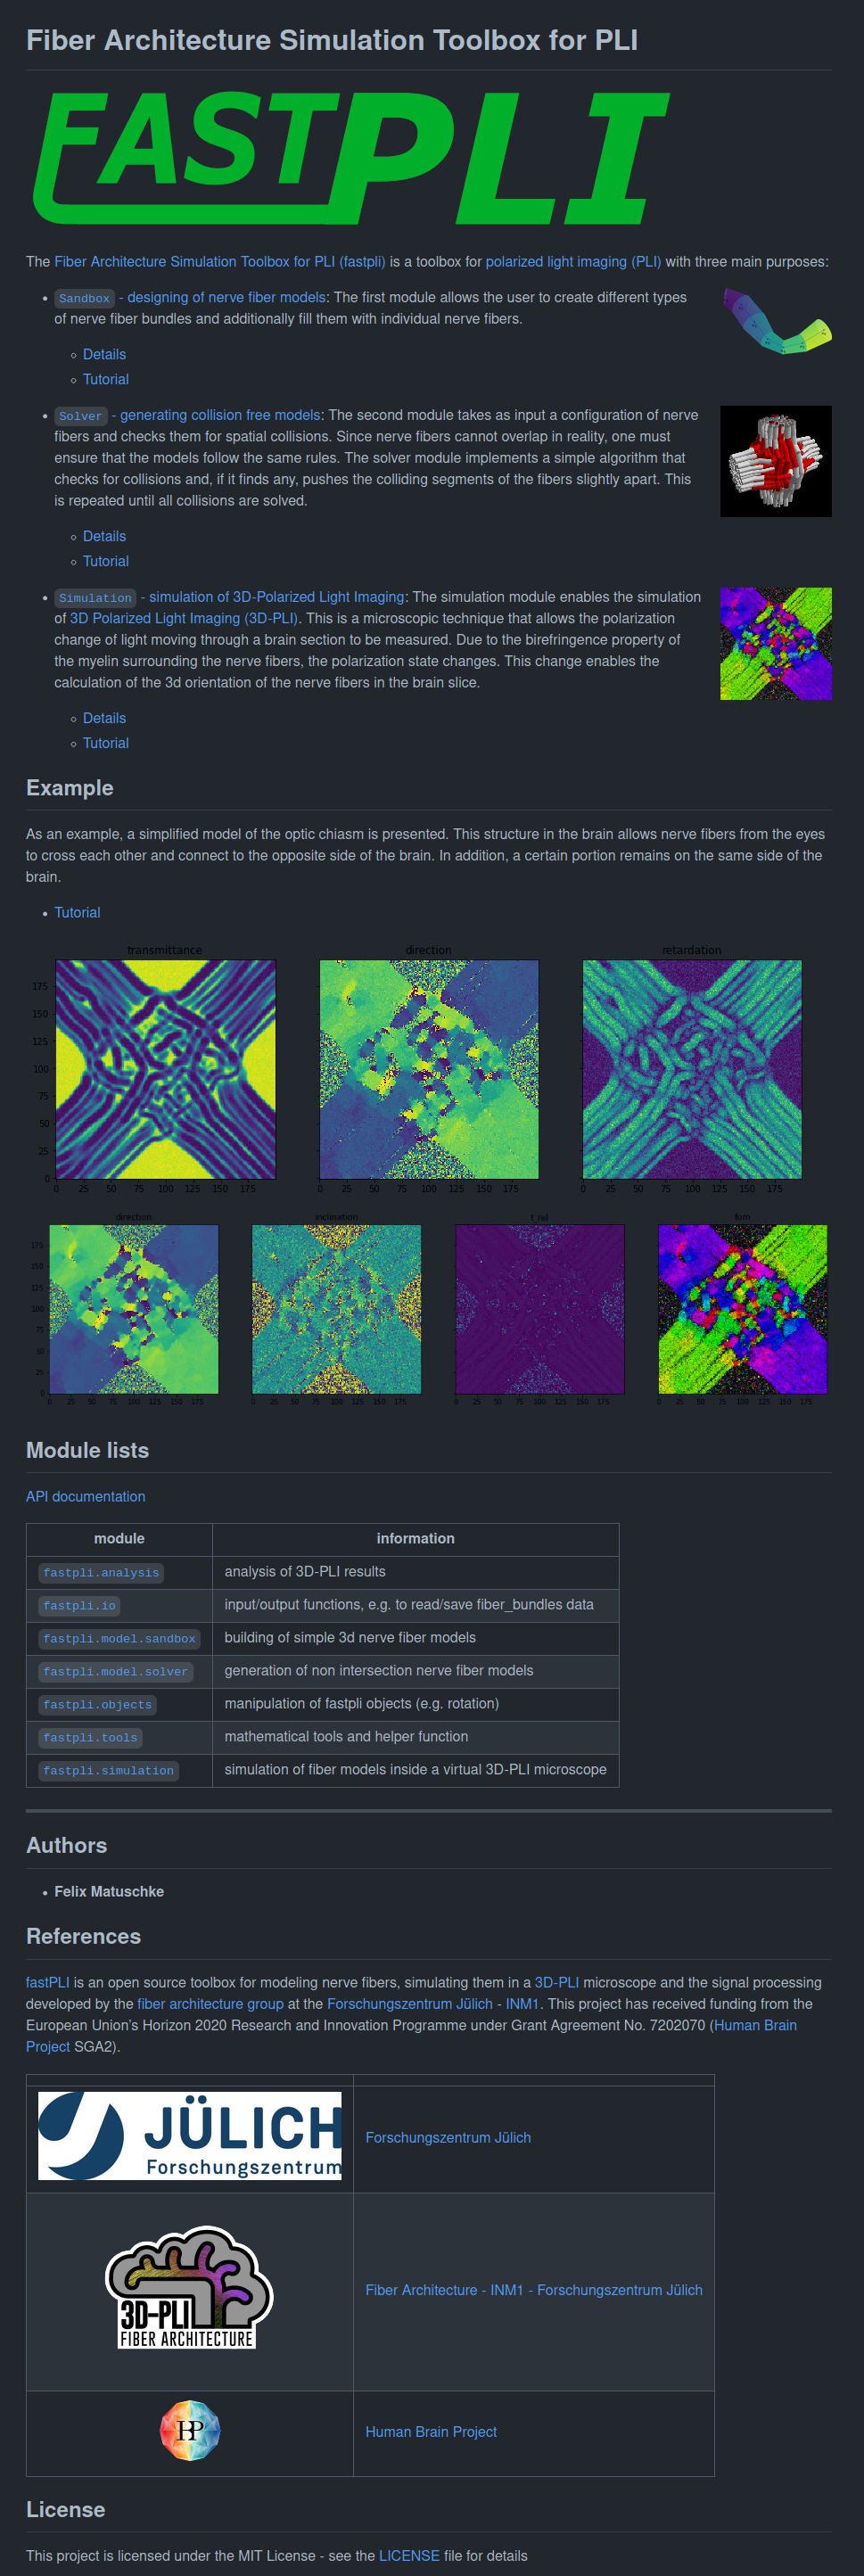
\includegraphics[valign=T,trim=0 1300 0 0, clip]{gfx/fastpli/fastpli_wiki.png} &
 	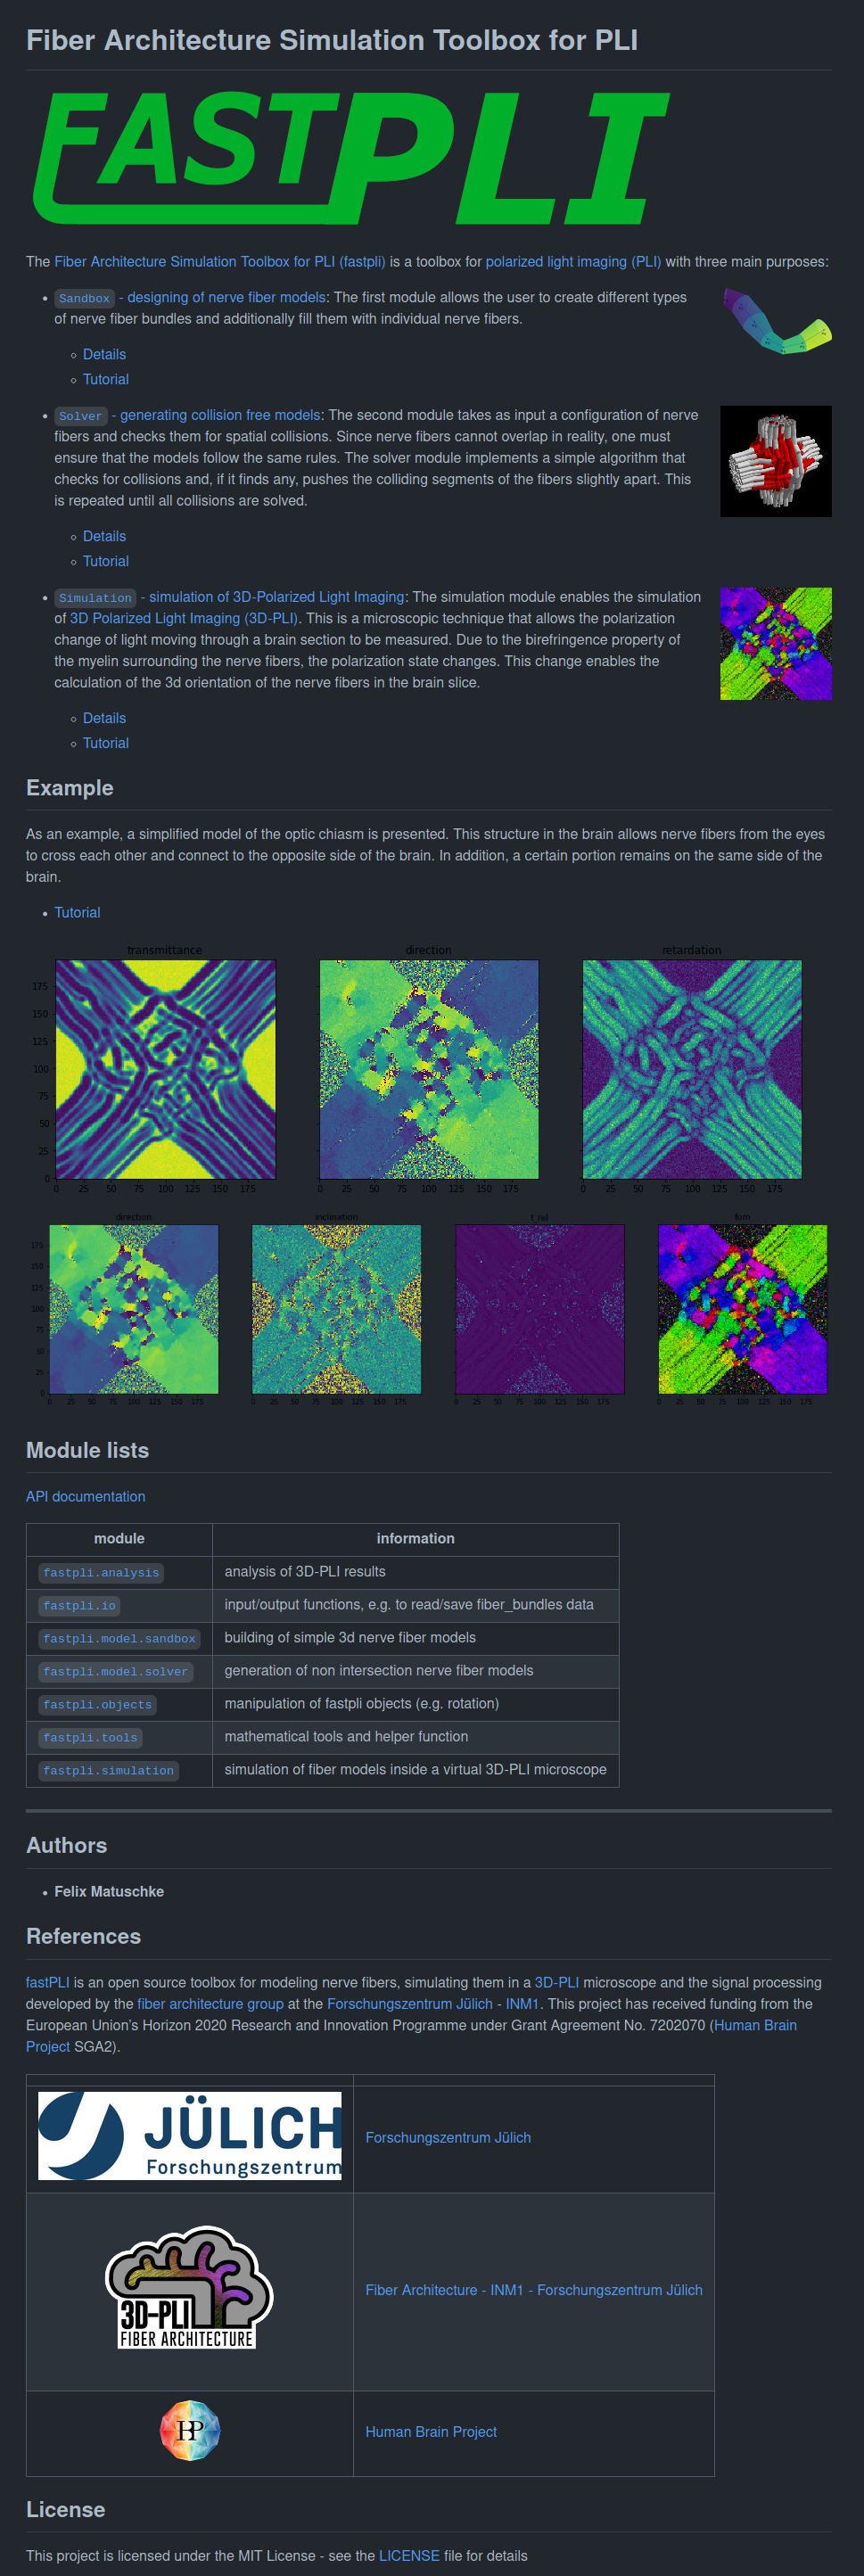
\includegraphics[valign=T,trim=0 0 0 1580, clip]{gfx/fastpli/fastpli_wiki.png} \\
    \end{tabular}
    }}
	\caption{\dummy{}}
	\label{fig:fastpli_wiki}
\end{figure}
% 
These docstrings also are used for an automatic release of a \ac{API} documentation\footnote{\url{https://3d-pli.github.io/fastpli/}}.
Additionally a wiki page describing the main funcionalities is available, which was also part of the review process for the publication in \textit{the Journal of Open Source Software (JOSS)} \cite{Matuschke2021} \footnote{Review open accessible under \url{https://github.com/openjournals/joss-reviews/issues/3042}}.
% 
To help the user with a fast ... process, executable python scribs as well as jupyter notebooks are as tutorials available.
A combined example of the overall package based on the optical chiasm is accessible as the last part.
\\
% 
To provide a fully tested software, each package and its main methods is automatic tested for each push with the automatic github action\footnote{They are \eg{} used for automatic build, test and deployment of the software and documentations.}.
These use the two latest Ubuntu long term support version (18.04 LTS and 20.04 LTS) and the most commonly used python3 version (3.6 and 3.8) to provide a wide range of automatic tested version.
Additionally the \textit{Github actions} run all tests, check the tutorial files, check the codes format and linting to be consistent and publish the documentations.
% 
Currently only Linux builds are supported, however for current windows version the \ac{WSL} probides a fully functional Linux Kernel inside Windows which can run the same ...
Current MacOS version are not automatic supported, however due to the minimalistic style of the \ac{fastPLI} package, the ... should be functional with minimal changes.
% 
% 
%  
\section{modules}
% 
\begin{lstfloat}[!ht]
\lstset{style=python}
\begin{lstlisting}
import fastpli
''' __version__
'''

import fastpli.analysis
''' affine_transformation
    epa
    images
    rofl
'''

import fastpli.io
''' fiber_bundles
'''

import fastpli.model.sandbox
''' fill
    shape
'''

import fastpli.model.solver
''' class Solver
    __solver.cpython.so
    _solver.py
'''

import fastpli.objects
''' fiber
    fiber_bundle
    fiber_bundles
'''

import fastpli.simulation
''' class Simpli
    __generation.cpython.so
    __simulation.cpython.so
    _simpli.py
    optic
'''

import fastpli.tools
''' label_converter
    rotation
'''
\end{lstlisting}
\caption[Overview \fastpli{} package]{Overview \fastpli{} package with containing modules}
% 	\label{alg:simulation}
\end{lstfloat}
% 
% 
%  
\subsection{fastpli.analysis}
\begin{lstfloat}[!ht]
\lstset{style=python}
\begin{lstlisting}
import fastpli.analysis
fastpli.analysis.affine_transformation
    # apply affine transformations to images (e.g. untilt)
fastpli.analysis.epa
    # analysis of 2d PLI images
fastpli.analysis.images
    # analysis/generation of color images (FOM, VectorImages, ...)
fastpli.analysis.rofl
    # analysis tilted PLI images
\end{lstlisting}
\caption{\code{fastpli.analysis}}
% 	\label{alg:simulation}
\end{lstfloat}
% 
% 
%  
\subsection{fastpli.io}
\begin{lstfloat}[!ht]
\lstset{style=python}
\begin{lstlisting}
import fastpli.io
fastpli.io.fiber_bundles
    # io operations for dat-files and hdf5-files
    # for the fiber_bundles format.
\end{lstlisting}
\caption{\code{fastpli.io}}\label{alg:fastpli.io}
\end{lstfloat}
% 
\paragraph{fiber\_bundles.py} contains io routines (see \cref{alg:fastpli.io}) for reading and saving fiber\_bundles into dat-files or hdf5-files. dat-files are text files which have to following structure as in \cref{alg:dat-file}. This dataformat is used to be as exchange friendly as possible for new users. \hdf{} files on the other hand are a binary dataformat \cite{hdf5}, where the individual datasets are arange in datacontainers, like the file explorer (see \cref{alg:hdf5}). The data contains 4d arrays, which are explained in \cref{sec:nerve_fiber_representation}.
% 
\begin{lstfloat}[!ht]
\lstset{style=common,morecomment=[l][\color{syntax_green}]{<-},}
\begin{lstlisting}
-6.55 -18.93 -64.98 3.75 <- x y z r
-5.73 -14.89 -63.37 3.4
-4.42 -13.66 -58.95 3.05
    <- empty line indicates new fiber
-1.96 -10.07 -52.5 2.92
-1.03 -9.4 -48.62 2.93

    <- two empty lines indicates new fiber bundle
3.4 -4.02 -44.76 3.11
6.22 -1.04 -42.45 3.26
\end{lstlisting}
\caption{exemplary dat-file format. Commets are currently not allowed and are only for the readers eyes.}\label{alg:dat-file}
\end{lstfloat}
% 
\begin{lstfloat}[!ht]
\lstset{style=common}
\begin{lstlisting}
GROUP "/" { # fiber_bundles path
  GROUP "0" { # id of fiber_bundle
      DATASET "0" { # id of fiber
         DATATYPE  H5T_IEEE_F64LE
         DATASPACE  SIMPLE { ( 3, 4 ) / ( 3, 4 ) }
         DATA {
         (0,0): -6.55, -18.93, -64.98, 3.75,
         (1,0): -5.73, -14.89, -63.37, 3.4,
         (2,0): -4.42, -13.66, -58.95, 3.05,
         }
      }
      DATASET "1" { # id of fiber
         DATATYPE  H5T_IEEE_F64LE
         DATASPACE  SIMPLE { ( 2, 4 ) / ( 2, 4 ) }
         DATA {
         (3,0): -1.96, -10.07, -52.5, 2.92,
         (4,0): -1.03, -9.4, -48.62, 2.93,
         }
      }
  }
  GROUP "1" { # id of fiber_bundle
      DATASET "0" { # id of fiber
         DATATYPE  H5T_IEEE_F64LE
         DATASPACE  SIMPLE { ( 2, 4 ) / ( 2, 4 ) }
         DATA {
         (0,0): 3.4, -4.02, -44.76, 3.11,
         (1,0): 6.22, -1.04, -42.45, 3.26,
         }
      }
  }
}
\end{lstlisting}
\caption{exemplary hdf5-file format.} \label{alg:hdf5}
\end{lstfloat}
% 
% 
% 
\subsection{fastpli.model.sandbox}
\begin{lstfloat}[!ht]
\lstset{style=python}
\begin{lstlisting}
import fastpli.model.sandbox
fastpli.model.sandbox.fill
    # filling of trajectaries with seed points as fiber_bundles
fastpli.model.sandbox.build
    # building of geometries
\end{lstlisting}
\caption{\code{fastpli.model.sandbox}}
% 	\label{alg:simulation}
\end{lstfloat}
% 
% 
% 
\subsection{fastpli.model.solver}
\begin{lstfloat}[!ht]
\lstset{style=python}
\begin{lstlisting}
import fastpli.model.solver
fastpli.model.solver.Solver
    # Class wrapper for C++ class.
    # Solves any 3d configurations of fibers to a non colliding ...
\end{lstlisting}
\caption{\code{fastpli.model.solver}}
% 	\label{alg:simulation}
\end{lstfloat}
% 
% 
% 
\subsection{fastpli.simulation}
\begin{lstfloat}[!ht]
\lstset{style=python}
\begin{lstlisting}
import fastpli.simulation
fastpli.simulation.Simpli
    # Class wrapper for C++ class.
    # Generatoes:
    #   - discretisied Tissue Volume
    #   - 3D PLI images
    #   - analysis of resultss
\end{lstlisting}
\caption{\code{fastpli.simulation}}
% 	\label{alg:simulation}
\end{lstfloat}
% 
% 
% 
\subsection{fastpli.tools}
\begin{lstfloat}[!ht]
\lstset{style=python}
\begin{lstlisting}
import fastpli.tools
fastpli.tools.label_converter
    # conversion of discretisied tissue to 
    # maxwell-solver input format
fastpli.tools.rotation
    # rotation matricies for 3d rotaions
\end{lstlisting}
\caption{\code{fastpli.tools}}
% 	\label{alg:simulation}
\end{lstfloat}
% 
% 
% 
\section{Dependencies}
% 
\paragraph{Python:}
\begin{description}
\item[numpy:] Base N-dimensional array package \cite{2019arXiv190710121V}\\
\url{https://numpy.org/}
\item[scipy:] Fundamental library for scientific computing \cite{2019arXiv190710121V}\\
\url{https://www.scipy.org/} 
\item[numba:] Acceleration of Python Functions \cite{Lam2015}\\
\url{https://numba.pydata.org/}
\item[mpi4py:] MPI for Python \cite{Dalcn2005, Dalcn2008, Dalcin2011}\\
\url{https://bitbucket.org/mpi4py/mpi4py/src/master/}
\item[h5py:] HDF5 for Python \cite{collette_python_hdf5_2014, hdf5}\\
\url{https://www.h5py.org/}
\end{description}
% 
\paragraph{C++:}
\begin{description}
\item[MPI:] Message Passing Interface \cite{message2015mpi}\\
\url{https://www.mpi-forum.org/}
\item[OpenMP:] Open Multi-Processing, API for multi-platform shared memory multiprocessing programming \cite{dagum1998openmp}\\
\url{https://www.openmp.org/}
\item[OpenGL:] Open Graphics Library \cite{khronos}\\
\url{www.opengl.org}
\item[Pybind11:] Seamless operability between C++11 and Python \cite{pybind11}\\ \url{https://github.com/pybind/pybind11} 
\end{description}
%